

\section{Vorstellung des Ergebnisses}

(TODO!): Julian schreibt die Übersicht hierzu.

Einleitung mit eher detailiertem Überblick über das Spiel.

Gerne alle Funktionen benennen, nichts erklären. Überblick verschaffen. 


Dazu Spielablaufskizze abarbeiten (Die Zeichnung(\ref{fig:2022-01-08-Spielablauf-Chart}) und Erläuterung erklären)

\begin{figure}[H]
    \centering
    \caption[]{08.01.2022: Diagram: Seitenaufbau und Spielablauf}
    \label{fig:2022-01-08-Spielablauf-Chart}
    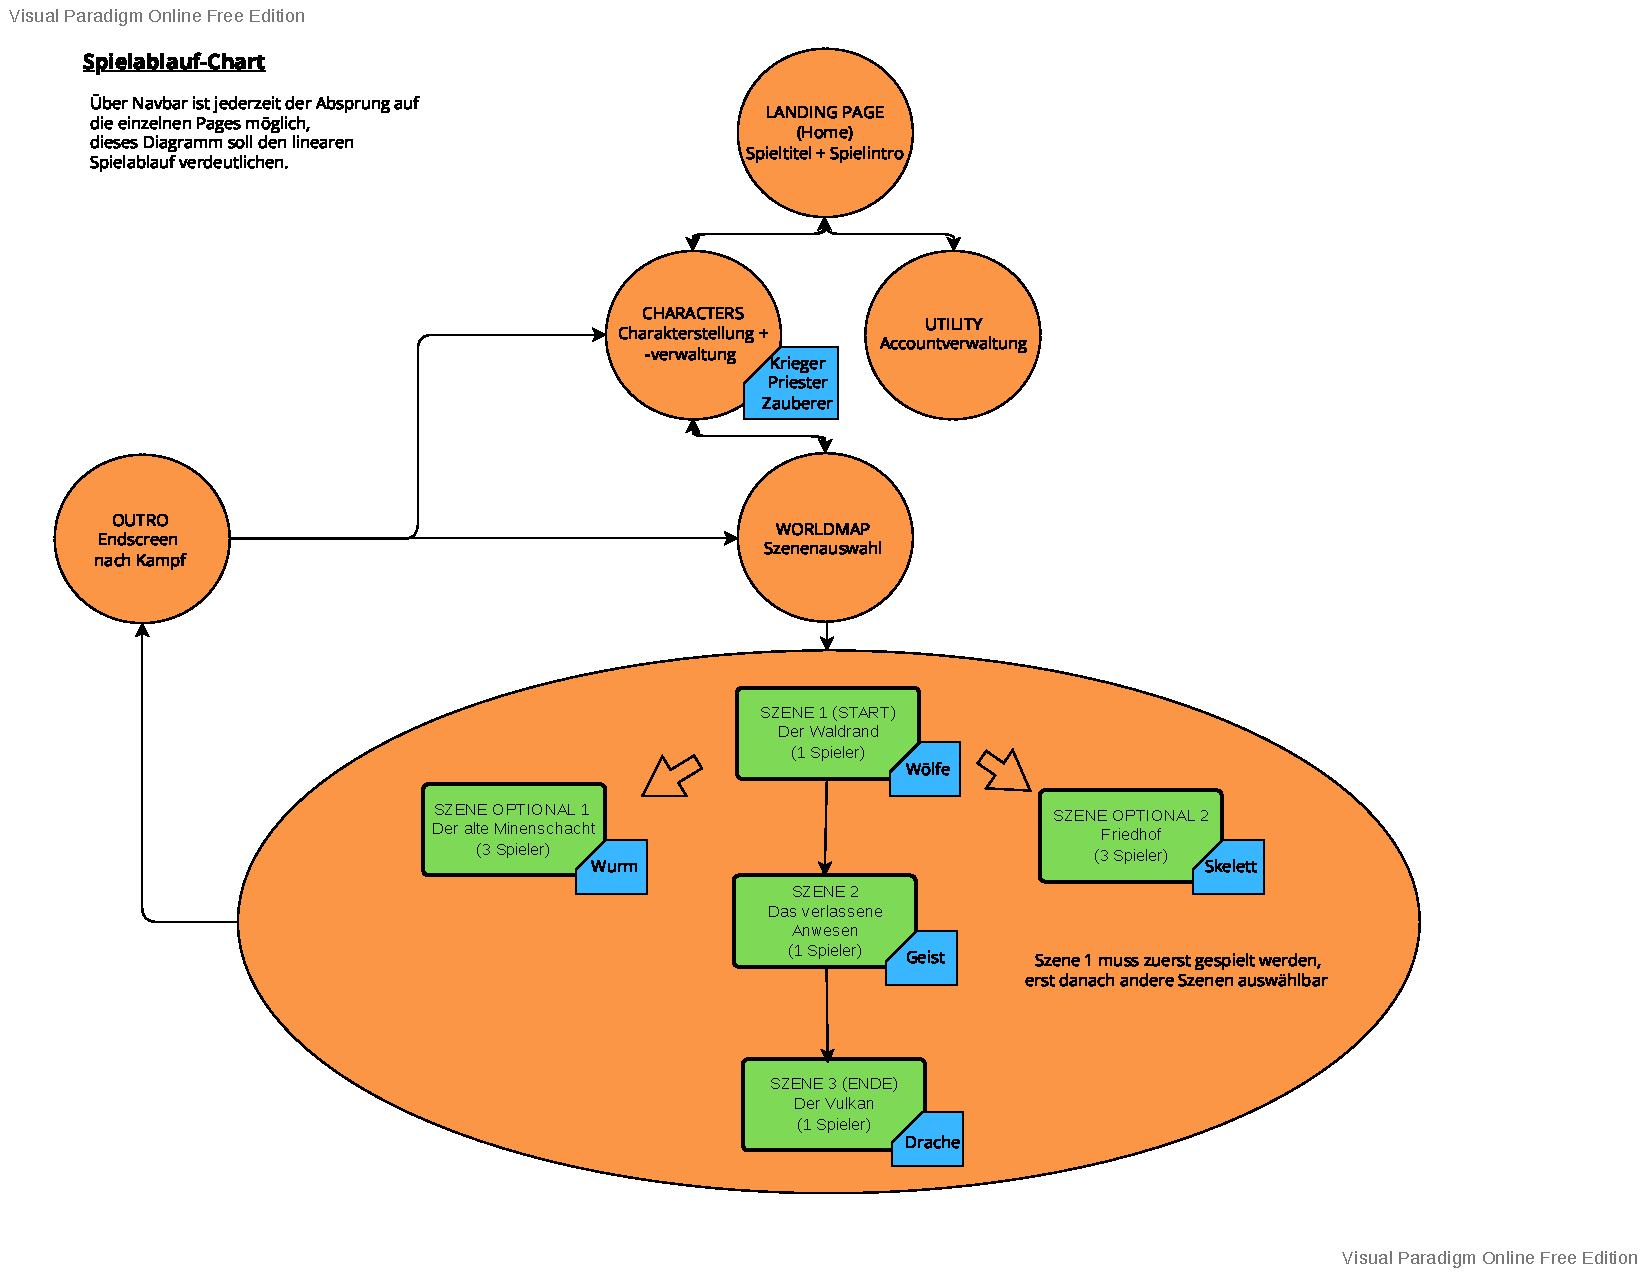
\includegraphics[width=1\textwidth]{2022-01-08-Spielablauf-Chart}
\end{figure}


(keine 5 Seiten)

